%%%%%%%%%%%%%%%%%%%%%%%%%%%%%%%%%%%%%%%%%
% Beamer Presentation
% LaTeX Template
% Version 1.0 (10/11/12)
%
% This template has been downloaded from:
% http://www.LaTeXTemplates.com
%
% License:
% CC BY-NC-SA 3.0 (http://creativecommons.org/licenses/by-nc-sa/3.0/)
%
%%%%%%%%%%%%%%%%%%%%%%%%%%%%%%%%%%%%%%%%%

%----------------------------------------------------------------------------------------
%	PACKAGES AND THEMES
%----------------------------------------------------------------------------------------

\documentclass[t]{beamer}

\mode<presentation> {

% The Beamer class comes with a number of default slide themes
% which change the colors and layouts of slides. Below this is a list
% of all the themes, uncomment each in turn to see what they look like.

%\usetheme{default}
%\usetheme{AnnArbor}
%\usetheme{Antibes}
%\usetheme{Bergen}
%\usetheme{Berkeley}
%\usetheme{Berlin}
%\usetheme{Boadilla}
%\usetheme{CambridgeUS}
%\usetheme{Copenhagen}
%\usetheme{Darmstadt}
%\usetheme{Dresden}
%\usetheme{Frankfurt}
%\usetheme{Goettingen}
%\usetheme{Hannover}
%\usetheme{Ilmenau}
%\usetheme{JuanLesPins}
%\usetheme{Luebeck}
\usetheme{Madrid}
%\usetheme{Malmoe}
%\usetheme{Marburg}
%\usetheme{Montpellier}
%\usetheme{PaloAlto}
%\usetheme{Pittsburgh}
%\usetheme{Rochester}
%\usetheme{Singapore}
%\usetheme{Szeged}
%\usetheme{Warsaw}

% As well as themes, the Beamer class has a number of color themes
% for any slide theme. Uncomment each of these in turn to see how it
% changes the colors of your current slide theme.

%\usecolortheme{albatross}
%\usecolortheme{beaver}
%\usecolortheme{beetle}
%\usecolortheme{crane}
%\usecolortheme{dolphin}
%\usecolortheme{dove}
%\usecolortheme{fly}
%\usecolortheme{lily}
%\usecolortheme{orchid}
%\usecolortheme{rose}
%\usecolortheme{seagull}
%\usecolortheme{seahorse}
%\usecolortheme{whale}
%\usecolortheme{wolverine}

%\setbeamertemplate{footline} % To remove the footer line in all slides uncomment this line
%\setbeamertemplate{footline}[page number] % To replace the footer line in all slides with a simple slide count uncomment this line

%\setbeamertemplate{navigation symbols}{} % To remove the navigation symbols from the bottom of all slides uncomment this line
}

\usepackage{graphicx} % Allows including images
\usepackage{booktabs} % Allows the use of \toprule, \midrule and \bottomrule in tables

%----------------------------------------------------------------------------------------
%	TITLE PAGE
%----------------------------------------------------------------------------------------

\title[]{Electronic Hardware Design} % The short title appears at the bottom of every slide, the full title is only on the title page

\author{Josh Johnson} % Your name
\institute[] % Your institution as it will appear on the bottom of every slide, may be shorthand to save space
{ CSides, September 2019\\ % Your institution for the title page
\medskip
\textit{} % Your email address
}
\date{13/9/2019} % Date, can be changed to a custom date

\begin{document}

\begin{frame}
\titlepage % Print the title page as the first slide
\end{frame}

%----------------------------------------------------------------------------------------
%	PRESENTATION SLIDES
%----------------------------------------------------------------------------------------
\begin{frame}
\frametitle{Overview}
\vspace{-20pt}
\begin{columns}
	\column{.4\textwidth}
	\begin{itemize}
		\item What and why?
		\item Schematic Capture
		\item PCB Layout
		\item Ordering Boards
		\item Assembly
		\item Mechanical Design
		\item Firmware
		\item Profit?
	\end{itemize}
	
	\column{.59\textwidth}
	\begin{figure}
		\includegraphics[width=0.9\linewidth]{csidesKB.jpg}
	\end{figure}
	
\end{columns}
\end{frame}
%----------------------------------------------------------------------------------------
\begin{frame}
\frametitle{What and Why?}
I wanted to build something to help with CAD \\[10pt]

\begin{itemize}
	\item Reprogrammable - able to send HID codes natively 
	\item Rotary Encoders - at least two
	\item RGB LEDs
	\item Cheap
\end{itemize}
\vspace{10pt}
Nothing available, so time to build my own!
\end{frame}
%----------------------------------------------------------------------------------------
\begin{frame}
\frametitle{Block Diagram}

\begin{figure}
	\centering
	\includegraphics[width=0.9\linewidth]{blockDiag.PNG}
	\includegraphics[width=0.9\linewidth]{blockDiagParts.PNG}
\end{figure}
\end{frame}
%----------------------------------------------------------------------------------------
\begin{frame}
\frametitle{Reference Designs}
We have picked our parts, but how do we figure out the schematic? \\[10pt]

\begin{itemize}
	\item Adafruit / Sparkfun Breakout Boards
	\item Evaluation Boards
	\item Application Notes
	\item Datasheet
\end{itemize}
\vspace{10pt}
With a reference design in hand, time to draw up the schematic
\end{frame}
%----------------------------------------------------------------------------------------
\begin{frame}[t]
\frametitle{EDA tool of choice: KiCad}

A Cross Platform and Open Source Electronic Design Automation Suite

\begin{columns}
	\column{.69\textwidth}
	\begin{itemize}
		\item KiCad - project manager
		\item Eeschema – schematic capture
		\item Pcbnew - layout program
		\item GerbView - gerber viewer
		\item Bitmap2Component - import images to PCB
	\end{itemize}
	
	
	\column{.3\textwidth}
	\begin{figure}
		\includegraphics[width=1\linewidth]{kikeycad.png}
		Image: @Chris\_Gammell
	\end{figure}
	
\end{columns}
\end{frame}
%----------------------------------------------------------------------------------------
\begin{frame}
\frametitle{Schematic Capture}
\vspace{-20pt}
\begin{columns}
	\column{.40\textwidth}
	\begin{itemize}
		\item Abstract representation of circuit
		\item Abstract representation of components 
		\item Drawn for ease of understanding
		\item Communicates purpose
		\item Documents design!
	\end{itemize}
	
	
	\column{.59\textwidth}
	\begin{figure}
		\includegraphics[width=0.8\linewidth]{circuit_diagram.png}
	\end{figure}
\end{columns}
\end{frame}
%----------------------------------------------------------------------------------------
\begin{frame}
\frametitle{Schematic Capture}
Key Steps:
\begin{itemize}
	\item Symbol creation
	\item Symbol placement
	\item Connect everything with wires
	\item Electrical rule check (ERC)
	\item Footprint association 
	\item Bill of Materials (BOM) generation
\end{itemize}
\end{frame}
%----------------------------------------------------------------------------------------
\begin{frame}
\frametitle{PCB Layout}
\begin{itemize}
	\item Physical representation of circuit
	\item Physical representation of components 
	\item Layout conforms to electrical and mechanical requirements 
\end{itemize}
	
	\begin{figure}
		\includegraphics[width=0.9\linewidth]{ice40.png}
	\end{figure}

\end{frame}
%----------------------------------------------------------------------------------------
\begin{frame}
\frametitle{Determine Manufacturer}
\begin{itemize}
	\item Manufacturers have design rules for the smallest feature sizes they can manufacture
	\item PCB thickness, colour, material, trace/space, surface finish, and physical dimensions all alter cost
	\item Figure out who will manufacture the boards before layout, or it may come back to bite you
\end{itemize}
\end{frame}
%----------------------------------------------------------------------------------------
\begin{frame}
\frametitle{PCB Stackup}
\begin{figure}
	\includegraphics[width=0.8\linewidth]{crossSection2.jpg}
\end{figure}
Image: @GregDavill
\end{frame}
%---------------------------------------------------------------------------------------
\begin{frame}
\frametitle{Key Design Rules}
\begin{figure}
	\includegraphics[width=0.7\linewidth]{lintekCu.png}
\end{figure}
\begin{itemize}
	\item Min track width / spacing (C / D)
	\item Min drill size (Not Shown)
	\item Min annular ring (A)
\end{itemize}
More: \url{http://www.lintek.com.au/wordpress/wp-content/uploads/Design-Capabilities-v2.7.pdf}
\end{frame}
%----------------------------------------------------------------------------------------
\begin{frame}
\frametitle{PCB Layout}
Key Steps:
\begin{itemize}
	\item Configure design rules and board setup based on manufacturer guidelines
	\item Place connectors, mounting holes, other mechanical components 
	\item Place electronic components
	\item Route critical nets
	\item Route power
	\item Route everything else
	\item Add decorative features
	\item Run design rule check (DRC)
	\item Export Gerbers
	\item Generate iBOM Pick and Place 	
\end{itemize}
\end{frame}
%----------------------------------------------------------------------------------------
\begin{frame}
\frametitle{Ordering Boards}
\begin{itemize}
	\item Check Gerbers in GerbView
	\item Zip up Gerbers
	\item Upload to manufacturer
	\item Choose PCB options
	\item Place order
	\item Don't forget to order parts!
\end{itemize}
\end{frame}
%----------------------------------------------------------------------------------------
\begin{frame}
\frametitle{Assembly}
\begin{figure}
	\includegraphics[width=\linewidth]{assembly/assm0.JPG}
\end{figure}
\end{frame}
%----------------------------------------------------------------------------------------
\begin{frame}
\frametitle{Assembly}
\begin{figure}
	\includegraphics[width=\linewidth]{assembly/assm1.JPG}
\end{figure}
\end{frame}
%----------------------------------------------------------------------------------------
\begin{frame}
\frametitle{Assembly}
\begin{figure}
	\includegraphics[width=\linewidth]{assembly/assm2.JPG}
\end{figure}
\end{frame}
%----------------------------------------------------------------------------------------
\begin{frame}
\frametitle{Assembly}
\begin{figure}
	\includegraphics[width=\linewidth]{assembly/assm3.JPG}
\end{figure}
\end{frame}
%----------------------------------------------------------------------------------------
\begin{frame}
\frametitle{Assembly}
\begin{figure}
	\includegraphics[width=\linewidth]{assembly/assm4.JPG}
\end{figure}
\end{frame}
%----------------------------------------------------------------------------------------
\begin{frame}
\frametitle{Assembly}
\begin{figure}
	\includegraphics[width=\linewidth]{assembly/assm5.JPG}
\end{figure}
\end{frame}
%----------------------------------------------------------------------------------------
\begin{frame}
\frametitle{Assembly}
\begin{figure}
	\includegraphics[width=\linewidth]{assembly/assm6.JPG}
\end{figure}
\end{frame}
%----------------------------------------------------------------------------------------
\begin{frame}
\frametitle{Assembly}
\begin{figure}
	\includegraphics[width=\linewidth]{assembly/assm7.JPG}
\end{figure}
\end{frame}
%----------------------------------------------------------------------------------------
\begin{frame}
	\frametitle{Assembly}
	\begin{figure}
		\includegraphics[width=\linewidth]{assembly/assm8.JPG}
	\end{figure}
\end{frame}
%----------------------------------------------------------------------------------------
\begin{frame}
	\frametitle{Assembly}
	\begin{figure}
		\includegraphics[width=\linewidth]{assembly/assm11.JPG}
	\end{figure}
\end{frame}
%----------------------------------------------------------------------------------------
\begin{frame}
	\frametitle{Assembly}
	\begin{figure}
		\includegraphics[width=\linewidth]{assembly/assm12.JPG}
	\end{figure}
\end{frame}
%----------------------------------------------------------------------------------------
\begin{frame}
	\frametitle{Assembly}
	\begin{figure}
		\includegraphics[width=\linewidth]{assembly/assm9.JPG}
	\end{figure}
\end{frame}
%----------------------------------------------------------------------------------------
\begin{frame}
	\frametitle{Assembly}
	\begin{figure}
		\includegraphics[width=\linewidth]{assembly/assm10.JPG}
	\end{figure}
\end{frame}
%----------------------------------------------------------------------------------------
\begin{frame}
\frametitle{Assembly}
\begin{figure}
	\includegraphics[width=\linewidth]{assembly/assm13.JPG}
\end{figure}
\end{frame}
%----------------------------------------------------------------------------------------
\begin{frame}
\frametitle{Assembly}
\begin{figure}
	\includegraphics[width=\linewidth]{assembly/assm14.JPG}
\end{figure}
\end{frame}
%----------------------------------------------------------------------------------------
\begin{frame}
\frametitle{Assembly}
\begin{figure}
	\includegraphics[width=\linewidth]{assembly/assm15.JPG}
\end{figure}
\end{frame}
%----------------------------------------------------------------------------------------
\begin{frame}
\frametitle{Assembly}
\begin{figure}
	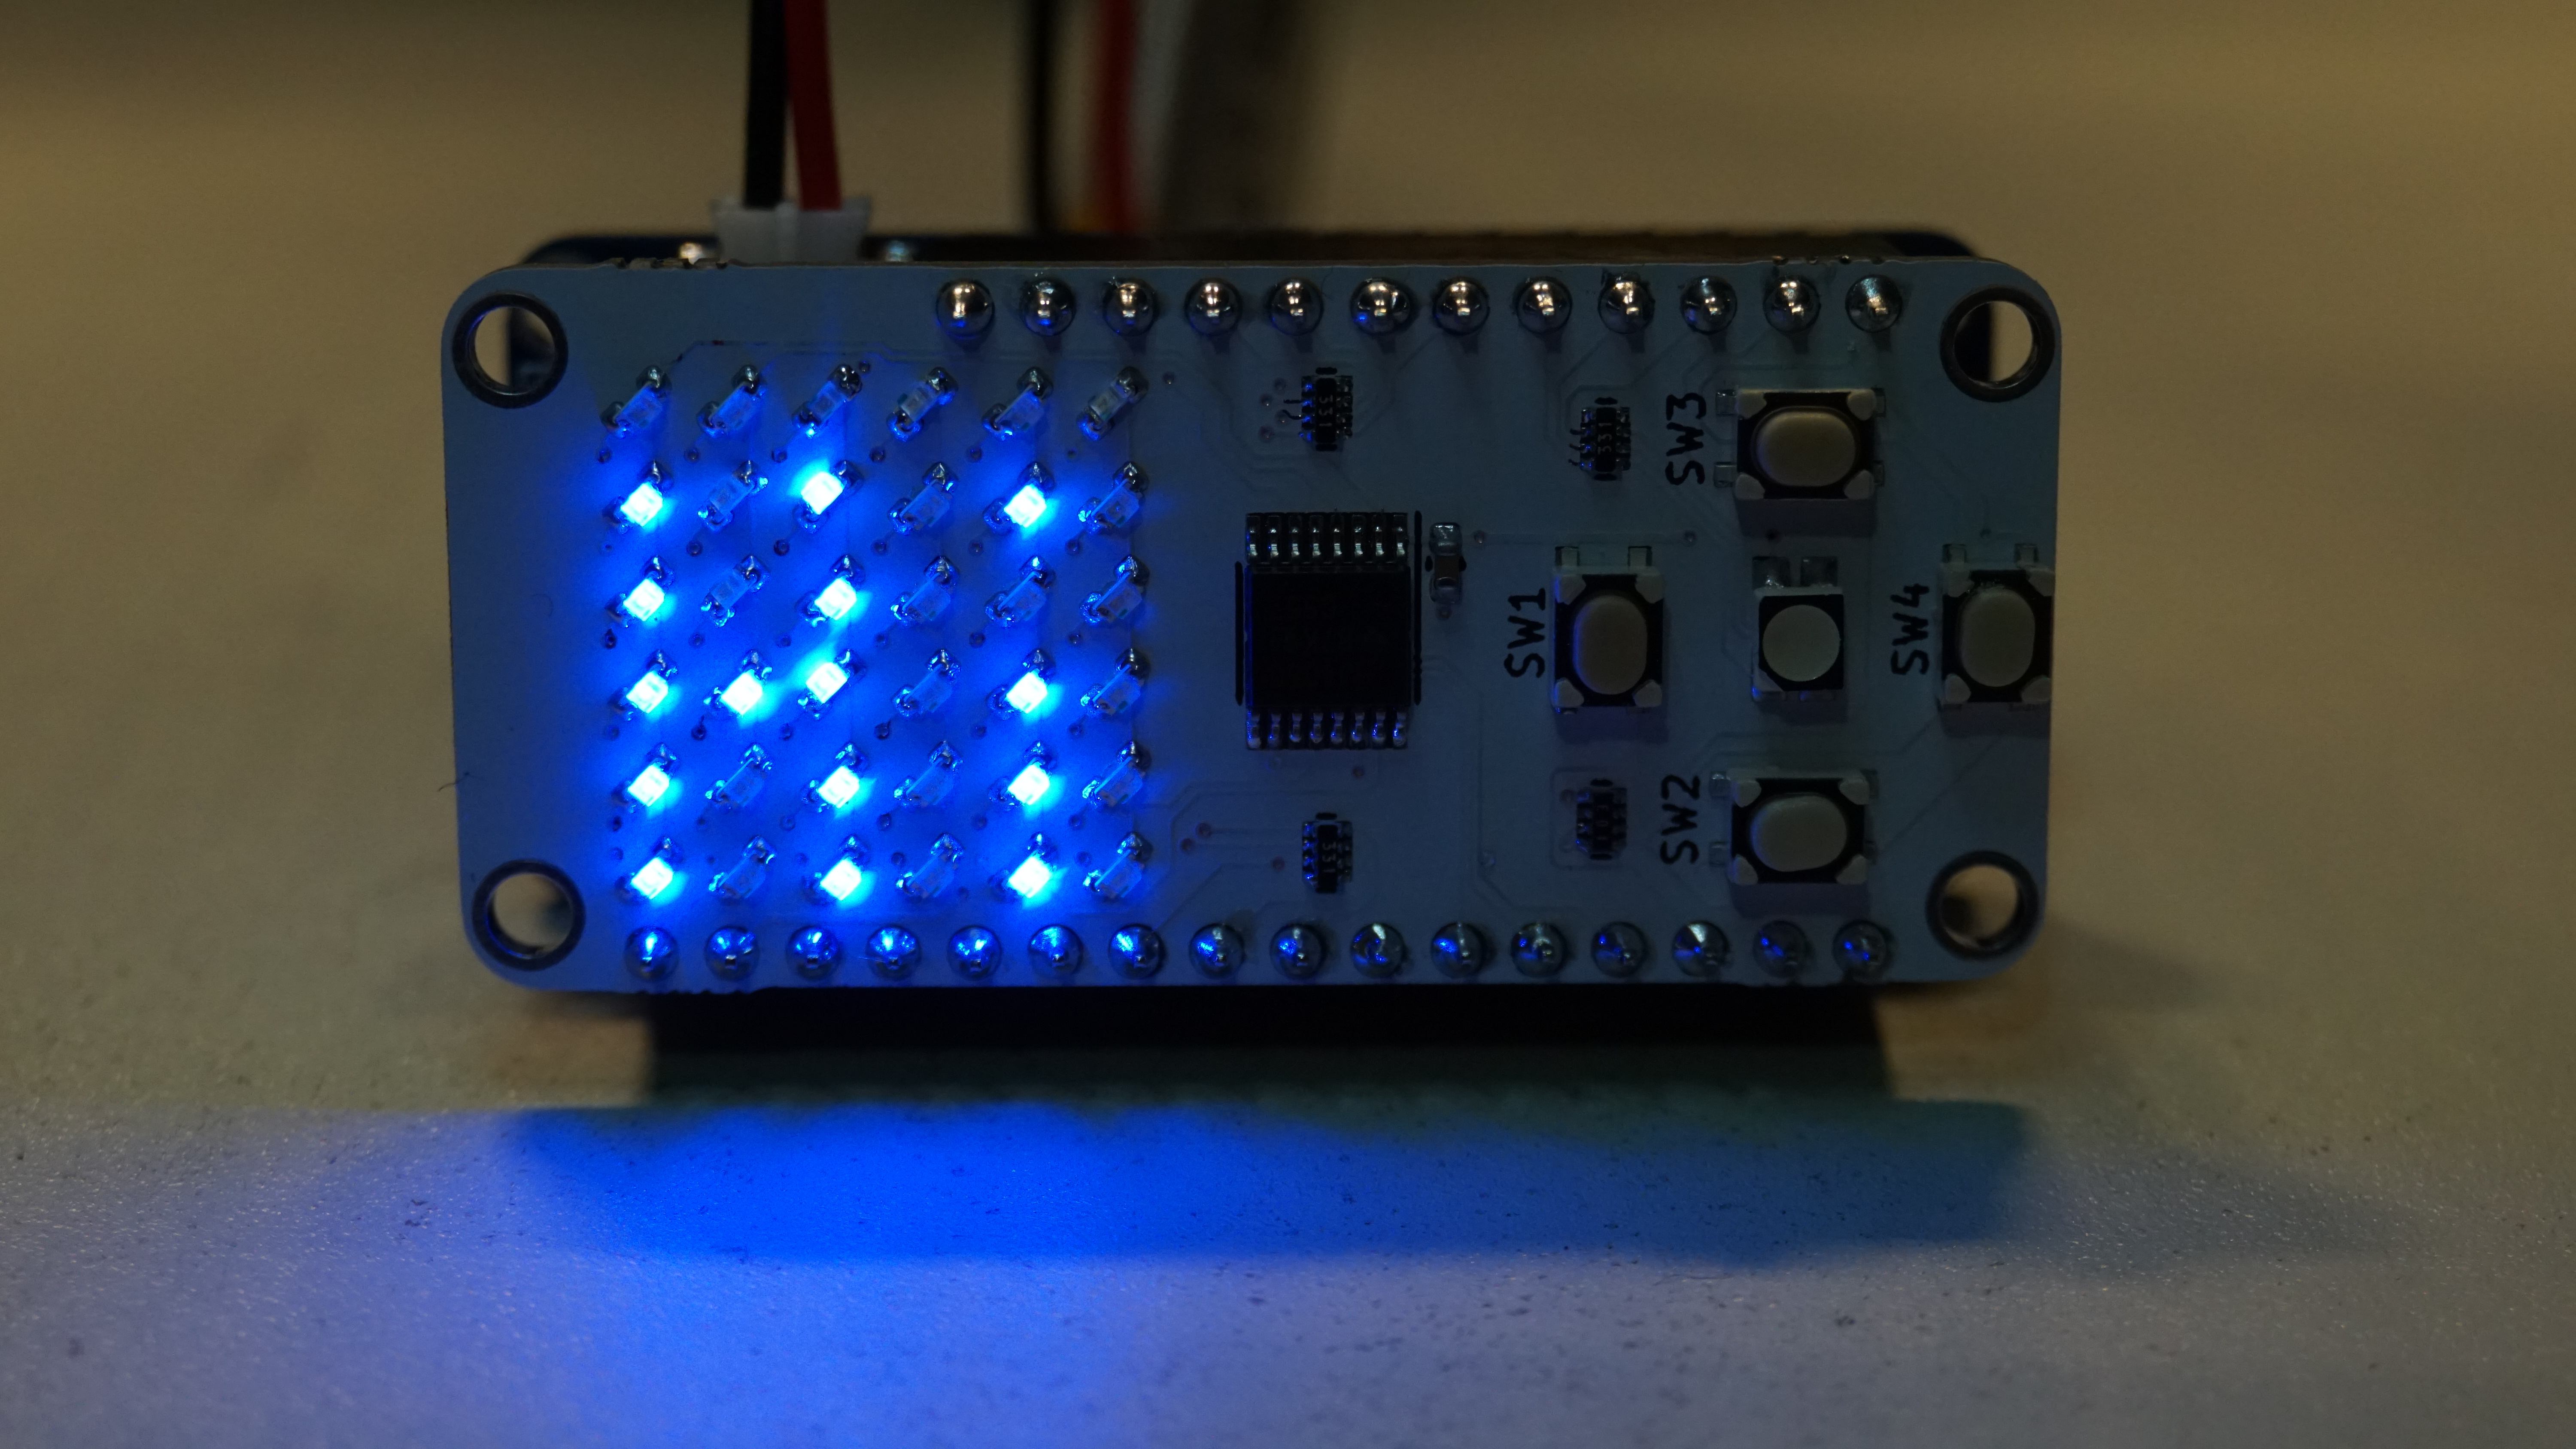
\includegraphics[width=\linewidth]{assembly/assm16.JPG}
\end{figure}
\end{frame}
%----------------------------------------------------------------------------------------
\begin{frame}
\frametitle{Mechanical Design}
Circuit boards are nice to look at, but sometimes they need an enclosure
\begin{itemize}
	\item Laser cutting
	\item 3D printing
	\item COTS enclosures
	\item PCB as a custom faceplate
\end{itemize}
\vspace{10pt}
Easiest way to design / ensure fit - export PCB from KiCad to MCAD\\[10pt]
You can also import .dxf from MCAD into KiCad, and use that for mechanical design
\end{frame}
%----------------------------------------------------------------------------------------
\begin{frame}
\frametitle{Firmware}
We have assembled the board, but we now need to program it. How?
\begin{itemize}
	\item Unlike an Arduino, new ICs typically lack a bootloader
	\item We need a programming header on the board to flash firmware
	\item Header may also be used for debug
\end{itemize}
\begin{columns}
	\column{.5\textwidth}
	\centering
	\includegraphics[width=\linewidth]{kbprog.jpg}
	\includegraphics[width=\linewidth]{usbasp.jpg}
	\column{.49\textwidth}
	\centering
	\includegraphics[width=0.9\linewidth]{vnaprog.jpg}
	\includegraphics[width=0.9\linewidth]{avrpogo.jpg}
\end{columns}
\end{frame}
%----------------------------------------------------------------------------------------
\begin{frame}
\frametitle{Keyboard Firmware}
Current Configuration
\begin{itemize}
	\item Arduino Caterina Bootloader
	\item Running QMK firmware
	\item Sends unused HID codes over USB
	\item AutoHotKey converts these into desired key presses, depending on open window
	\item Allows for macros to be set for KiCad / Chrome / Fusion 360 etc
\end{itemize}
HID codes could also be hard coded to desired combinations on device
\end{frame}
%----------------------------------------------------------------------------------------
\begin{frame}
\frametitle{Final Product}
\begin{figure}
	\centering
	\includegraphics[width=\linewidth]{keyboards.jpg}
\end{figure}
\begin{itemize}
	\item I now have a custom keyboard which is not only great for CAD, but is used for multiple applications on my computer
	\item During the build, learnt of / how powerful QMK is, so bought a full size keyboard which runs QMK firmware
	\item Now have two completely reprogrammable keyboards, which not only increase productivity, but have been configured to help mitigate RSI issues 
\end{itemize}
\end{frame}
%----------------------------------------------------------------------------------------
\begin{frame}
\frametitle{Profit?}
\end{frame}
%----------------------------------------------------------------------------------------
\begin{frame}
\frametitle{Shitty Add-Ons}
\begin{columns}[c]
	\column{.6\textwidth}
	\centering
		\includegraphics[width=0.8\linewidth]{sao.jpg}
		\includegraphics[width=0.7\linewidth]{hackerchix.jpg}
	
	\column{.39\textwidth}
	\centering
	\includegraphics[width=\linewidth]{joshsao.jpg}
	Images: @mrtwinkletwink, @BSidesCbr
\end{columns}
\end{frame}
%----------------------------------------------------------------------------------------
\begin{frame}
\frametitle{Shitty Add-On}
Design your own!\\[10pt]
Check out the \texttt{SAO/SAO101.pro} KiCad project\\
Schematic capture is complete, components are ready to be laid out, just need to connect the dots!\\[10pt]

\end{frame}
%----------------------------------------------------------------------------------------
\begin{frame}
\frametitle{Questions?}
Slides and Files: \url{github.com/joshajohnson/CBRhardware}\\[10pt]
README contains links if you want to learn more\\[10pt]
Happy to help out anyone designing a board, feel free to get in touch. \\[10pt]
I have lots of circuit boards on me, please say hello!
\vspace{5mm}

Email: josh@joshajohnson.com\\
Twitter: @\textunderscore joshajohnson\\
BSidesCbr Slack: josh\\
\vspace{4mm}
\end{frame}
\end{document} 